\pstart 
[158 v\textsuperscript{o}] Witsen\protect\index{Namensregister}{\textso{Witsen,} Nicolaes 1641\textendash 1717} \edtext{fol.}{\lemma{Witsen}\Afootnote{ \textit{ (1) }\ pag. \textit{ (2) }\ fol. \textit{ L}}} 139. \textit{Schipsbow in bestier} \edlabel{itadevelisstart}ita\edtext{}{{\xxref{itadevelisstart}{itadevelisend}}\lemma{ita}\Bfootnote{Von ita de velis bis haest hefft vgl. \textsc{N. Witsen}, \cite{00153}a.a.O., S.~139.}} de velis\protect\index{Sachverzeichnis}{velum}: \textit{Het }\textit{Zeildoeck}\protect\index{Sachverzeichnis}{Zeil\textendash doeck}\textit{ nu, werdt gesponnen van fijn geklopte }\textit{Hennip}\protect\index{Sachverzeichnis}{hennep}\textit{. De maet der }\textit{zeilen}\protect\index{Sachverzeichnis}{zeil}\textit{ werdt mede wel geschickt, na het gebruik, waer to de }\textit{shepen}\protect\index{Sachverzeichnis}{schip}\textit{ gebeziget sullen werden.} \edtext{Auff}{\lemma{}\Afootnote{Auff \textit{ erg.} \textit{ L}}} jachtschiffa\protect\index{Sachverzeichnis}{Jacht} und die auß seyn, umb ander Zu verfolgen, viel \edtext{seile}{\lemma{viel}\Afootnote{ \textit{ (1) }\ sel \textit{ (2) }\ seile \textit{ L}}}. Kleine Schiffe\protect\index{Sachverzeichnis}{Schiff} seilen beßer ins gemin als große, weil in ihnen die Seegel\protect\index{Sachverzeichnis}{Segel} großer nach proportion. Denn wenn sie in grossen schiffen\protect\index{Sachverzeichnis}{Schiff} auch nach proportion so große \edtext{weren}{\lemma{große}\Afootnote{ \textit{ (1) }\ wurd \textit{ (2) }\ weren \textit{ L}}}, wie in kleinen, weren sie zu groß, und nicht wohl zu regiren. Die Segel\protect\index{Sachverzeichnis}{Segel} m\"{u}ßen nicht zu starck gespannt seyn, \edtext{[sondern]}{\lemma{}\Afootnote{sonden\textit{\ L \"{a}ndert Hrsg.}}} es ist beßer daß ihnen der Wind einige Rundheit gebe denn also faßet der wind beßer im seil, und gibt dem tuch mehr bewegung (+ denn nichts laufft an der seite ab 
%Zeitz auskommentiert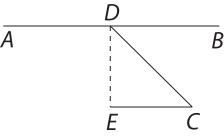
\includegraphics[width=0.2\textwidth]{images/38_158v1} 
denn wenn \textit{AB} der segel\protect\index{Sachverzeichnis}{Segel} eine rechte lini, so dreibt ihn nur der perpendicularis \textit{DE}, \edtext{nicht}{\lemma{\textit{DE},}\Afootnote{ \textit{ (1) }\ ist \textit{ (2) }\ nicht \textit{ L}}} die parallela \textit{CE}. Wenn es aber rund, treibt ihn \textit{CE} auch +). Die Seeleute halten daf\"{u}r, daß die vordersten Seegel\protect\index{Sachverzeichnis}{Segel} dem schiff\protect\index{Sachverzeichnis}{Schiff} den meisten fortgang\protect\index{Sachverzeichnis}{Schiff-Bewegung} geben, und geben \edtext{diese}{\lemma{geben}\Afootnote{ \textit{ (1) }\ zu \textit{ (2) }\ als \textit{ (3) }\ vor \textit{ (4) }\ diese \textit{ L}}} ursach, daß als da der wind das schiff\protect\index{Sachverzeichnis}{Schiff} gleichsam ziehet, und hinden oder in der mitten allein \textit{douwt}, item, das der wind in den Vorseegelen\protect\index{Sachverzeichnis}{Vorsegel} \textit{de baeren der Zee} be{\ss}er schneidet, weil er n\"{a}her. Doch hat man nicht viel zu Seegel\protect\index{Sachverzeichnis}{Segel} vorn zu machen, damit das schiff\protect\index{Sachverzeichnis}{Schiff} nicht dadurch komme sich zu b\"{u}cken (\textit{kome te bocken}). Man h\"{a}lt auch dafur da{\ss} die obere Seegel\protect\index{Sachverzeichnis}{Segel} mehr macht geben als die untere, die weil der mast\protect\index{Sachverzeichnis}{Mast} ein Heber\protect\index{Sachverzeichnis}{Hebel} ist, und de{\ss}en fu{\ss} der Punct der ruhe. \textit{Dit ongemaeck echter slepen deze boven-Zeilen\protect\index{Sachverzeichnis}{zeil} mede}, datse \textit{lichter} von \textit{boven neer} kommen, \textit{en in hart weer niet gebruyckt konnen werden}. Die Seegel\protect\index{Sachverzeichnis}{Segel} vermindern sich gegen die hohe zu, damit sie nicht oben zuviel wind faßen und das schiff\protect\index{Sachverzeichnis}{zeil} machen umbschlagen, oder vorn zu sehr eindauchen; item daß die masten\protect\index{Sachverzeichnis}{Mast} oben weniger vertragen als unten. Mit halbem winde tragen alle Seegel\protect\index{Sachverzeichnis}{Segel}, welches mit Vorwind nicht geschehen kan, und bey Vorwind \textit{geit man het groote Zeil\protect\index{Sachverzeichnis}{Grootzeil} op} umb wind an die vorsegel\protect\index{Sachverzeichnis}{Vorsegel} zu geben.
\pend 
\pstart Darumb \edtext{wird}{\lemma{Darumb}\Afootnote{ \textit{ (1) }\ soll \textit{ (2) }\ wird \textit{ L}}} auch ein schiff\protect\index{Sachverzeichnis}{Schiff} mehr fart machen mit einem Seitenwind, als mit einem Vorwind, \edtext{(+ \textit{schoon niet all ten voordele} +)}{\lemma{Vorwind,}\Afootnote{ \textit{ (1) }\ ob gleich sol \textit{ (2) }\ (+ [...] +) \textit{ L}}} obschohn solche fart nicht in allen \edtext{vortheil hefft}{\lemma{allen}\Afootnote{ \textit{ (1) }\ zu ede \textit{ (2) }\ vortheil hefft \textit{ L}}}. Das hintere 3eckige Seegel\protect\index{Sachverzeichnis}{Segel} kan in fall der noth dem Steuer\protect\index{Sachverzeichnis}{Steuer} helffen, \textit{want men dit zeil\protect\index{Sachverzeichnis}{zeil} best zetten kan op de} streeck dar \textit{men heen will, en het Schip}\protect\index{Sachverzeichnis}{schip} nothw\"{a}ndig \textit{van achtern gestiert moot zijn. Dees} word \textit{by} Vorwind \textit{omgedraeit, en dwars} wanschappen \textit{tegen} den \textit{Mast}\protect\index{Sachverzeichnis}{Mast} geset, \textit{wanneer men grooten haest hefft}\edlabel{itadevelisend}. 
\pend 
\pstart \edtext{Es ist\edlabel{esiststart}}{{\xxref{esiststart}{esistend}}\lemma{Es ist}\Bfootnote{Von Es ist bis te vaeren vgl. \textsc{N. Witsen}, \cite{00153}a.a.O., S.~140.}} der Seele\"{u}te haupt regel keinen wind ohne nuzen zu verlieren und vorbeistreychen zu laßen. Dazu were guth, daß man beyderseits fl\"{u}gel ersinnen k\"{o}ndte. \textit{Hier toe zoude men vleugels wedersyts buiten boord konnen versinnen, gelijck men die by wijlen aen de Nocken van de Rees ziet geheckt, }\textit{Geiken}\protect\index{Sachverzeichnis}{Geiken}\textit{ en }\textit{Ly-Zeils}\protect\index{Sachverzeichnis}{Ly-Zeils}\textit{ genaemt welcke onder weinig breeder zeyn als boven. Dit geschiet in} \edtext{\textit{Jacht maecken}}{\lemma{\textit{Jacht}}\Afootnote{ \textit{ (1) }\ \textit{mach} \textit{ (2) }\ \textit{maecken} \textit{ L}}}\protect\index{Sachverzeichnis}{Jacht}\textit{, vlieden, en als, men groten haest hefft. }
\pend 
\pstart \textit{Onder aen de mars zeilen}\protect\index{Sachverzeichnis}{marszeil}\textit{ worden in zoo een }\edtext{\textit{geval}}{\lemma{\textit{een}}\Afootnote{ \textit{ (1) }\ \textit{gevall} \textit{ (2) }\ \textit{geval} \textit{ L}}}\textit{ wel mede }\textit{zeilen}\protect\index{Sachverzeichnis}{zeil}\textit{ aen gebonden die men fatzen }\edtext{\textit{noemt}}{\lemma{\textit{fatzen}}\Afootnote{ \textit{ (1) }\ \textit{neemt} \textit{ (2) }\ \textit{noemt} \textit{ L}}}\textit{, nevens een vin, achter by de }\textit{vlagge spil}\protect\index{Sachverzeichnis}{vlagge spil}. En Schiffer muß achtung geben, daß ein seegel\protect\index{Sachverzeichnis}{Segel} des anden wind nicht auff fange. Einige meinen das die Seegel\protect\index{Sachverzeichnis}{Segel} so sacksweise, \edtext{viel}{\lemma{sacksweise,}\Afootnote{ \textit{ (1) }\ den \textit{ (2) }\ viel \textit{ L}}} wind fangen, und den Lauff beschleinigen. 
\pend 
\clearpage 
\pstart \textit{Schepen}\protect\index{Sachverzeichnis}{schip}\textit{ nemen den meesten }\edtext{\textit{voortgang}}{\lemma{\textit{meesten}}\Afootnote{ \textit{ (1) }\ \textit{vortgang} \textit{ (2) }\ \textit{voortgang} \textit{ L}}}\protect\index{Sachverzeichnis}{schip\textendash voortgang}\textit{, als'er een greeps tows} wind, of \textit{back\-stags koelte is, en dat met twe of drie streecken van voorwind }\edtext{\textit{af:}}{\lemma{\textit{voorwind}}\Afootnote{ \textit{ (1) }\ \textit{aft} \textit{ (2) }\ \textit{af} \textit{ L}}}\textit{ want dus draegen de zeilen}\protect\index{Sachverzeichnis}{zeil} \edlabel{alle.start}\edtext{\textit{alle.}}{{\xxref{alle.start}{alle.end}}\lemma{\textit{alle.}}\Afootnote{ \textit{ (1) }\ \textit{Als} \textit{ (2) }\ \textit{als} \textit{ (3) }\ \textit{Alst} \textit{ L}}}
\pend 
\pstart \textit{Alst}\edlabel{alle.end} \textit{bij de wind gaet, kan men geen boven blinde gebruicken om dat het by zoo een gevall, te veel wabbert, en niet} stetvig \textit{genoegh gezet kan werden. Gelijck men noch dese, noch onder blinde in hart weer gebruicken kan}. In harten wetter machen sie das schiff\protect\index{Sachverzeichnis}{Schiff} zuviel eintauchen, und sind wegen der n\"{a}he beym Waßer nicht wohl zu regiren. 
\pend 
\pstart \textit{In storm word de }\textit{Bezaen}\protect\index{Sachverzeichnis}{Besan}\textit{ gebolt, en }\textit{Fock}\protect\index{Sachverzeichnis}{fok}\textit{ geset op }\textit{steven}\protect\index{Sachverzeichnis}{steven}\textit{.} 
\pend 
\pstart Je niedriger die Segel\protect\index{Sachverzeichnis}{Segel}, ie beßer sie regirt k\"{o}nnen werden und ie weniger sie lauffen \edtext{\textit{om}}{\lemma{lauffen}\Afootnote{ \textit{ (1) }\ umb \textit{ (2) }\ \textit{om} \textit{ L}}} \textit{van boven neer to geraecken}. Derowegen es ein guther fund seyn w\"{u}rde, wenn man das Seegelwerck\protect\index{Sachverzeichnis}{Segel} zur seiten aus zu stellen w\"{u}ste, anstatt daß es oben stehet. \edtext{Wie ungest\"{u}m}{\lemma{stehet.}\Afootnote{ \textit{ (1) }\ Hoe onstim \textit{ (2) }\ Wie ungest\"{u}m \textit{ L}}} es auch wehet, k\"{o}nnen die Bezaen\protect\index{Sachverzeichnis}{Besan} alzeit gef\"{u}hrt werden, \textit{is ook zelden onklaer}. In engen, und da man offt wenden mus gebraucht man allein die Voorseegel\protect\index{Sachverzeichnis}{Vorsegel}, \textit{met dese giert het schip\protect\index{Sachverzeichnis}{schip} minst}. Mit den vorseegeln\protect\index{Sachverzeichnis}{Vorsegel} wendet man das schiff\protect\index{Sachverzeichnis}{Schiff} vor den wind um\footnote{\textit{\"{U}ber} vor den wind: vor de wint om}, und mit den hinderseilen\protect\index{Sachverzeichnis}{achterzeil} by de wind op. Denn die weil das schiff\protect\index{Sachverzeichnis}{Schiff} auff seinen mittelpunct draeibar \edtext{is}{\lemma{draeibar}\Afootnote{ \textit{ (1) }\ ist \textit{ (2) }\ is \textit{ L}}}, das hinder theil \textit{bewogen werdende}, das voderste den gegenweg gehet, et contra. Daraus folgt daß de Bezaenen\protect\index{Sachverzeichnis}{Besan} der Schiffe\protect\index{Sachverzeichnis}{Schiff} \textit{by de wind doet gaen, en de blinde af} fallen. Die Seegel\protect\index{Sachverzeichnis}{Segel} werden hoch oder niedrig \textit{opgehaelt}, nach dem man große \edtext{vaert}{\lemma{große}\Afootnote{ \textit{ (1) }\ Vart \textit{ (2) }\ vaert \textit{ L}}} und mehr oder wenig windfang begehrt. Stracks ausgereckte und gespante Seegel\protect\index{Sachverzeichnis}{Segel} faßen den meisten Wind. \textit{Bordige} Seegel\protect\index{Sachverzeichnis}{Segel}, thun den wind \textit{ter zijden afspatten, en daerom goet om by de wind en met scherpe wind te vaeren}\edlabel{esistend}. \edtext{\textit{De Zeilen}\edlabel{dezeilenstart}}{{\xxref{dezeilenstart}{dezeilenend}}\lemma{\textit{De Zeilen}}\Bfootnote{Von De Zeilen bis zeilde vgl. \textsc{N. Witsen}, \cite{00153}a.a.O., S.~139.}}\protect\index{Sachverzeichnis}{zeil}, \textit{dienen niet al te strack of te bordig aen de raes gehecht te syn, maer op die wijse dat de wind daer in blaezende de zelvige eenige rontheit geefft, en dus vat de wind beter in het} \edtext{\textit{Zeil},}{\lemma{\textit{het}}\Afootnote{ \textit{ (1) }\ Seel, \textit{ (2) }\ \textit{Zeil}, \textit{ L}}} \textit{of kaen meer beweging aen het doeck} \edtext{\textit{over}}{\lemma{}\Afootnote{\textit{over} \textit{ erg.} \textit{ L}}} \textit{geven, en het schip}\protect\index{Sachverzeichnis}{schip} soll \textit{beter voortgang\protect\index{Sachverzeichnis}{schip\textendash voortgang} hebben. Ten waere men zeer scherp by te wind zeilde}\edlabel{dezeilenend}. 
\pend 
\pstart \edtext{Wann man\edlabel{wannmanstart}}{{\xxref{wannmanstart}{wannmanend}}\lemma{Wann}\Bfootnote{Von Wann man bis bringen solte vgl. \textsc{N. Witsen}, \cite{00153}a.a.O., S.~140.}} die fart st\"{u}tzen will, haelt \textit{men de }\textit{Mars-zeils}\protect\index{Sachverzeichnis}{marszeil}\textit{ op de rand of zeer laeg. }
\pend 
\pstart \textit{ Als }\edtext{\textit{man}}{\lemma{\textit{Als}}\Afootnote{ \textit{ (1) }\ \textit{men} \textit{ (2) }\ \textit{man} \textit{ L}}}\textit{ de }\textit{Shepen}\protect\index{Sachverzeichnis}{schip}\textit{ over staegh smiit, of tegen wind om laet gaen, moet men de }\textit{fock}\protect\index{Sachverzeichnis}{fok}\textit{ laeten loopen, ander sints loopt men gefahr von een uyl te vangen: of dat het }\textit{schip}\protect\index{Sachverzeichnis}{schip}\textit{ deist op zyn gat.}
\pend 
\pstart \textit{ Op droogten luysteren de }\textit{Schepen}\protect\index{Sachverzeichnis}{schip}\textit{ weinig na het }\textit{roer}\protect\index{Sachverzeichnis}{roer}\textit{ en dan moet men't }\textit{schip}\protect\index{Sachverzeichnis}{schip}\textit{ mit zeilen stueren, 't geen met ophaelen, laeten vallen, en }\edtext{\textit{dus}}{\lemma{\textit{en}}\Afootnote{ \textit{ (1) }\ \textit{daß} \textit{ (2) }\ \textit{dus} \textit{ L}}}\textit{ of zoo te stellen geschiet, na de konst van een ervaeren Zeeman. De Zee-lieden seggen}, daß es geschiht \textit{dat het zant zuigt, en het stuer}\protect\index{Sachverzeichnis}{stuur}\textit{ na zigh haelt.} Der wahrheit \"{a}hnlicher scheinet es zu seyn, daß die wenige distanz zwischen dem kiel\protect\index{Sachverzeichnis}{Kiel} und dem grund einen schnellen und großen umlauff von waßer verursacht, \textit{en en schielijcke waters} infall \textit{in het ledigh, 't }\edtext{\textit{welck}}{\lemma{\textit{'t}}\Afootnote{ \textit{ (1) }\ \textit{welch} \textit{ (2) }\ \textit{welck} \textit{ L}}} \textit{het }\textit{schip}\protect\index{Sachverzeichnis}{schip}\textit{ achter komt te maecken, het }\textit{roer}\protect\index{Sachverzeichnis}{roer}\textit{ ongeschickt doet schudden, en het }\textit{achter-schip}\protect\index{Sachverzeichnis}{achterschip} onmaetelich \textit{bewegen waer door het stueren bezwaerlijck} nootwendig fallen \textit{moet}. Es sind einige die rathen man solle alle seegel\protect\index{Sachverzeichnis}{Segel} auf einen schiff\protect\index{Sachverzeichnis}{Schiff} viereckt machen, oder gleichseitige dreyeck en die spalke met veele dwershouten, dus beter wind zullende vatten, welches meines bedenckens \edtext{mehr ungelegghet}{\lemma{mehr}\Afootnote{ \textit{ (1) }\ schaden \textit{ (2) }\ ungelegghet \textit{ L}}} als nuzen auffm schiff\protect\index{Sachverzeichnis}{Schiff} bringen solte\edlabel{wannmanend}.